\PassOptionsToPackage{usenames,dvipsnames,table,x11names}{xcolor}
\documentclass[11pt]{article}

%------------------------------------------------------
%                Math Packages
%------------------------------------------------------

%\usepackage[intlimits]{amsmath}
\usepackage{amsmath}
\usepackage{amssymb}
\usepackage{amsthm}
%\everymath{\displaystyle}
\usepackage{siunitx} % for SI units (e.g. C, degree)
\usepackage{bm} % bold for some math symbols
\usepackage{nicefrac} % for nicer fractions sometimes
\usepackage[thinc]{esdiff} % for derivatives
\usepackage{mathtools}

%------------------------------------------------------
%                Tikz and Pgfplots
%------------------------------------------------------

\usepackage{pgfplots}
\usepackage{tkz-euclide}
\pgfplotsset{compat=1.15}
\usetikzlibrary{arrows,shadows,positioning, calc, decorations.markings, hobby, quotes, angles, decorations.pathreplacing, intersections, matrix,backgrounds}
\usepgfplotslibrary{polar,colormaps,fillbetween}
\usepgflibrary{shapes.geometric}
%\usetkzobj{all}

%------------------------------------------------------
%                Formatting
%------------------------------------------------------

% COLORS ----------------------------------------------
%\usepackage[dvipsnames, table]{xcolor}
\usepackage{xcolor}

% FIGURES ---------------------------------------------
\usepackage{graphicx} % for importing images
\usepackage{subcaption} % for making subfigures
\usepackage[textfont=it]{caption} % changing style of figures
% labelfont=bf % sometimes use this too

% PAGE LAYOUT -----------------------------------------
%\linespread{1.3} % changes line spacing

\usepackage[a4paper, portrait, margin=1in]{geometry} % for changing layout of document
%\usepackage[a4paper, portrait, left=0.75in, right = 0.75in, top = 1in, bottom=1in]{geometry}

%\usepackage{indentfirst}
%\usepackage{parskip} % for not indenting paragraphs first
\usepackage{multirow} % having multiple rows
\usepackage{multicol} % having multiple columns
\renewcommand\labelitemi{$\vcenter{\hbox{\tiny$\bullet$}}$} % making bullets in \enumerate smaller
\usepackage[T1]{fontenc} % can combine \sc and \bf font
\usepackage{pdflscape} % for changing page orientation
\usepackage{afterpage} % to not have landscape page breaks
\usepackage{rotating} % rotating images in landscape

% LINKS -----------------------------------------------
\usepackage{etoolbox}
\makeatletter % <================================================
\patchcmd{\maketitle}%
  {\def\@makefnmark{\rlap{\@textsuperscript{\normalfont\@thefnmark}}}}%
  {\def\@makefnmark{\rlap{\@textsuperscript{\normalfont\color{blue}\@thefnmark}}}}%
  {}%success
  {}%failure
\makeatother % <=================================================
% for changing color of \thanks{} in title

\usepackage[hidelinks]{hyperref}
\hypersetup{
    colorlinks=true,
    linkcolor=black,
    filecolor=magenta,      
    urlcolor=black,
    citecolor=Blue4,
}

% LANGUAGES -------------------------------------------
\usepackage[english]{babel} % for correctly using english
\usepackage[utf8x]{inputenc} % compiling correctly
\usepackage{CJK} % using Chinese, Japanese, and Korean

% MISC ------------------------------------------------
\usepackage[normalem]{ulem} % for \sout
\usepackage{tikzsymbols} % for emojis
\usepackage{booktabs,eqparbox} % for tables
\usepackage{tabularx} % more customizable tables
\usepackage{verbatim} % for verbatim environment

% CITING ----------------------------------------------
\usepackage{apacite}
\newcommand{\citeay}[1]{\citeauthor{#1} \citeyear{#1}}

%------------------------------------------------------
%                Custom Commands
%------------------------------------------------------

\newcommand{\done}{\hfill $\square$}
\newcommand{\csch}{\mathrm{csch}}
\newcommand{\sech}{\mathrm{sech}}

%\newcommand{\dd}{\mathop{}\,\mathrm{d}}
\newcommand{\dd}{\,\mathrm{d}}

% COLOR CODING -----------------------------------------------
\newcommand{\code}[1]{\textcolor{Bittersweet}{\texttt{#1}}} % using for emphasizing variables, code, etc.
\newcommand{\mydef}[1]{\textcolor{SteelBlue3}{\textit{#1}}} % defining something

% VENN DIAGRAMS ----------------------------------------------
\def\firstcircle{(90:1.75cm) circle (2.5cm)}
\def\secondcircle{(210:1.75cm) circle (2.5cm)}
\def\thirdcircle{(330:1.75cm) circle (2.5cm)}
\def\sampspace{(-6,-4.25) rectangle (6,5)}  %Cartesian
%\def\sampspace{(225:7cm) rectangle (45:7cm)} %polar

% TO DO LIST -------------------------------------------------
\usepackage{enumitem}

\newlist{todolist}{itemize}{2}
\setlist[todolist]{label=$\square$}

\usepackage{pifont}
\newcommand{\cmark}{\ding{51}}%
\newcommand{\xmark}{\ding{55}}%
\newcommand{\fin}{\rlap{$\square$}{\raisebox{2pt}{\color{Green}{\large\hspace{1pt}\cmark}}}%
\hspace{-2.5pt}}
\newcommand{\wontfix}{\rlap{$\square$}{\color{red}{\large\hspace{1pt}\xmark}}}

% LADE STUFF -------------------------------------------------
\xdef\defsize{4}
\xdef\cursize{5}
\newcommand{\myscale}[1]{\defsize/#1}

%------------------------------------------------------
%                Custom Environments
%------------------------------------------------------

\usepackage{mdframed}

% EXERCISE -------------------------------------------------
\mdfdefinestyle{exercise}{
	backgroundcolor=black!10,roundcorner=8pt,hidealllines=true,nobreak
}

%\begin{mdframed}[style=exercise]
%\end{mdframed}

% MATHEMATICA ------------------------------------------------
\mdfdefinestyle{mathematica}{
	backgroundcolor=Tan!15,roundcorner=8pt,hidealllines=true,nobreak,fontcolor=Bittersweet
}

% R ---------------------------------------------------------
\mdfdefinestyle{R}{
	backgroundcolor=SteelBlue3!10, roundcorner=8pt, hidealllines=true, fontcolor=SteelBlue4
}

% R ---------------------------------------------------------
\mdfdefinestyle{python}{
	backgroundcolor=Green!15, roundcorner=8pt, hidealllines=true, fontcolor=Green
}

%------------------------------------------------------
%                      Layout
%------------------------------------------------------

% FORMATTING TITLES -----------------------------------
\usepackage{titlesec}
\titleformat*{\section}{\Large \bfseries} % changing section format
\titleformat*{\subsection}{%\color{SteelBlue3} 
\large \bf} % changing subsection format
%\setcounter{secnumdepth}{0} % sets title counter to 0

% PAGE HEADINGS ----------------------------------------------
\usepackage{fancyhdr}

\pagestyle{plain}
\fancyhf{}
\lhead{}
\chead{}
\rhead{}
\cfoot{\thepage}

\renewcommand{\headrulewidth}{0.2pt}
\renewcommand{\footrulewidth}{0pt}
\pagenumbering{gobble}

%%%%%%%%%%%%%%%%%%%%%%%%%%%%%%%%%%%%%%%%%%%%%%%%%%%%%%%
%%%%%%%%%%%%%%%%%%%%%%%%%%%%%%%%%%%%%%%%%%%%%%%%%%%%%%%

\usepackage{lipsum}

\begin{document}

%------------------------------------------------------
%                       Title
%------------------------------------------------------

\title{Tables for Report}
\author{Aiden Kenny and Danielle Solomon\\
Lamar University\\
4400 S M L King Jr Pkwy, Beaumont, TX 77705}
\date{Summer 2019}
\maketitle

%------------------------------------------------------
%                      Document
%------------------------------------------------------

\lipsum[1-2]

% want to put a table and images here

%%%%%%%%%%%%%% COLON

\afterpage{
\begin{landscape}
\begin{table}[p]
    \footnotesize
    \centering
    \def\arraystretch{1.5}

    \begin{tabularx}{0.971\linewidth}{lccccccccccc} \toprule
         & \multicolumn{3}{c}{No Clustering} & \multicolumn{4}{c}{$K$-means Clustering} & \multicolumn{4}{c}{Hierarchical Clustering} \\ 
         & \multicolumn{3}{c}{--} & \multicolumn{4}{c}{$K=9$} & \multicolumn{4}{c}{$K=7$} \\   
         \cmidrule(r){2-4} \cmidrule(lr){5-8} \cmidrule(l){9-12}
         % this is what has to be replaced with xtable
         & Lasso & Elastic Net & pcLasso & gLasso & sgLasso & cMCP & pcLasso & gLasso & sgLasso & cMCP & pcLasso \\ \midrule
        \multirow{2}{*}{Parameters} & $\lambda = 0.0642$ & $\lambda = 0.0853$ & $\lambda = 8.75$ & $\lambda = 0.00562$ & $\lambda = 0.0215$ & $\lambda = 0.0838$ & $\lambda = 35.32$ & $\lambda = 0.0621$ & $\lambda = 0.0194$ & $\lambda = 0.0813$ & $\lambda = 163.94$ \\ 
        & -- & $\alpha = 0.95$ &  $\texttt{rat} = 0.95$ & -- & $\alpha = 0.4$ & $\gamma = 30$ & $\texttt{rat} = 0.25$ & -- &  $\alpha = 0.05$ & $\gamma = 30$ & $\texttt{rat} = 0.95$ \\ 
        Deviance & 0.938 & 0.945 & 0.561 & 0.490 & 0.853 & 1.01 & 0.525 & 0.987 & 0.863 & 0.995 & 0.548 \\ 
        Misclass. & 6/31 & 6/31 & 5/31 & 12/31 & 7/31 & 6/31 & 5/31 & 8/31 & 11/31 & 6/31 & 3/31 \\ 
        Sig. Coef. &  16 &  19 &  30 &  49 &  29 &  11 &  30 &  20 & 461 &  11 &   7 \\ 
        Sig. Groups & -- & -- & -- &  3 &  2 &  4 &  9 &  1 &  1 &  4 &  6 \\ 
        %FPR & 4/11 & 4/11 & 3/11 & 7/11 & 6/11 & 4/11 & 3/11 & 4/11 & 11/11 & 4/11 & 2/11 \\ 
        %TPR & 18/20 & 18/20 & 18/20 & 15/20 & 19/20 & 18/20 & 18/20 & 16/20 & 20/20 & 18/20 & 19/20 \\ 
        AUC & 0.936 & 0.945 & 0.850 & 0.695 & 0.745 & 0.932 & 0.891 & 0.623 & 0.814 & 0.932 & 0.818 \\ 
        %
        \bottomrule
    \end{tabularx}
    %\caption{The performance of various models on the colon data set.}
    %\label{colon_tab}

\end{table}

\vspace{0.5cm}

\begin{figure}[p]
    \centering
    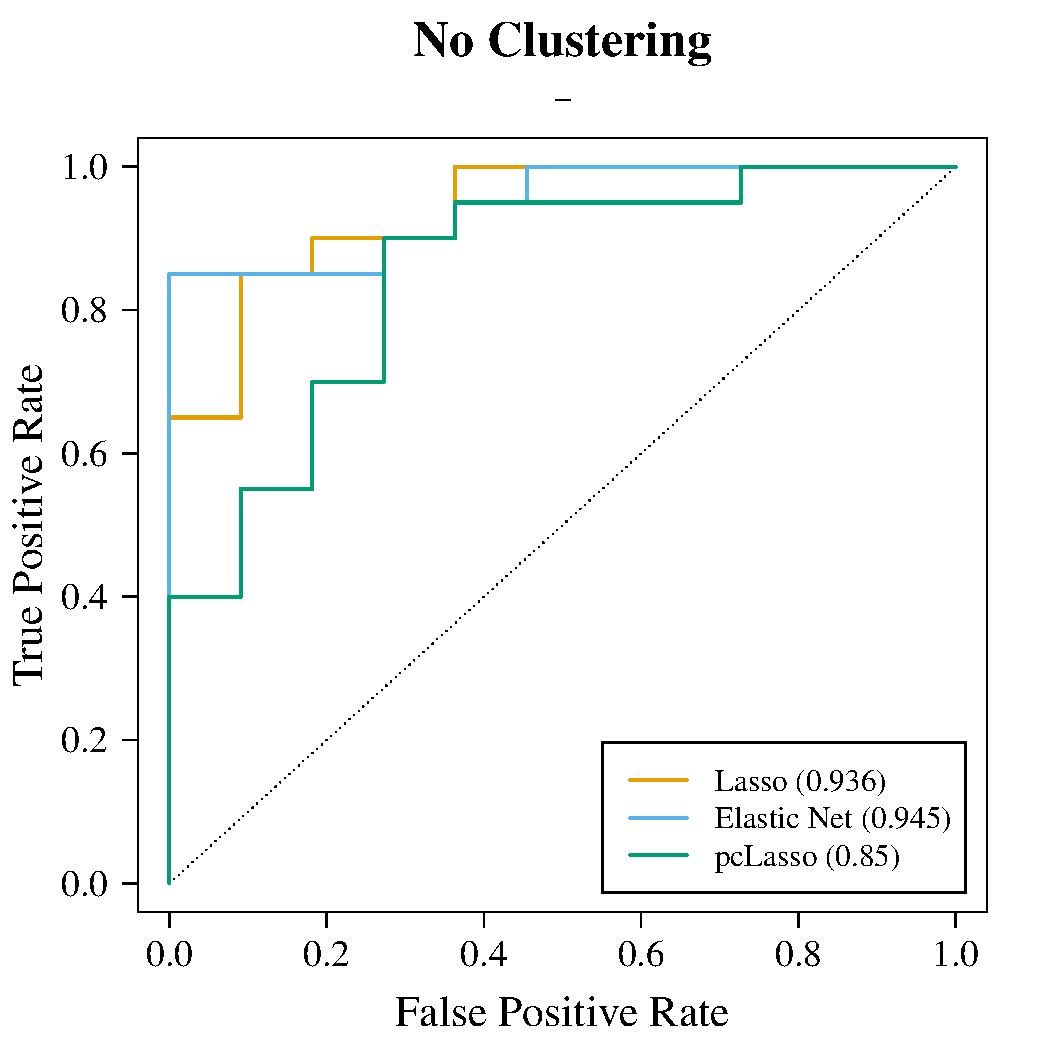
\includegraphics[width = 0.475\textwidth]{colon_ROC_no_n.pdf}
    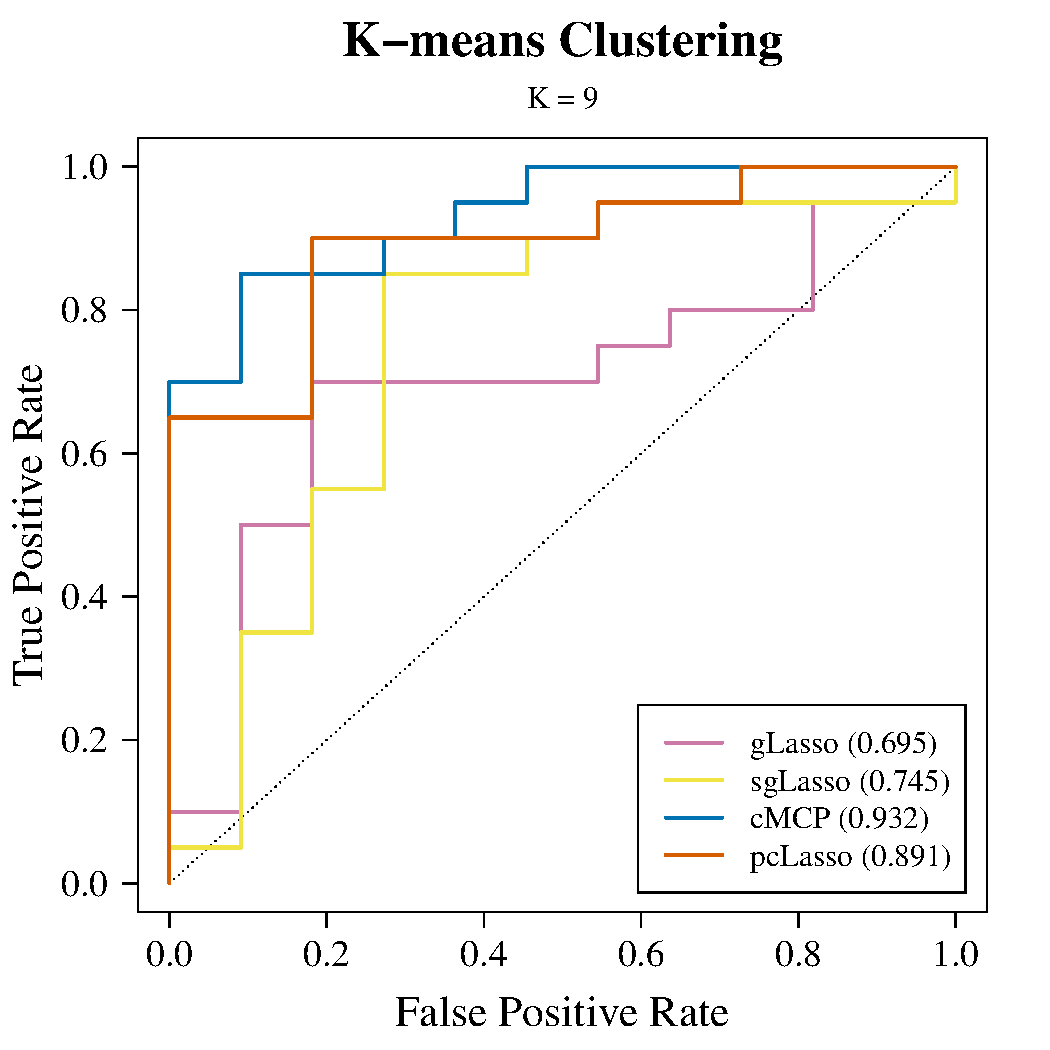
\includegraphics[width = 0.475\textwidth]{colon_ROC_k_n.pdf}
    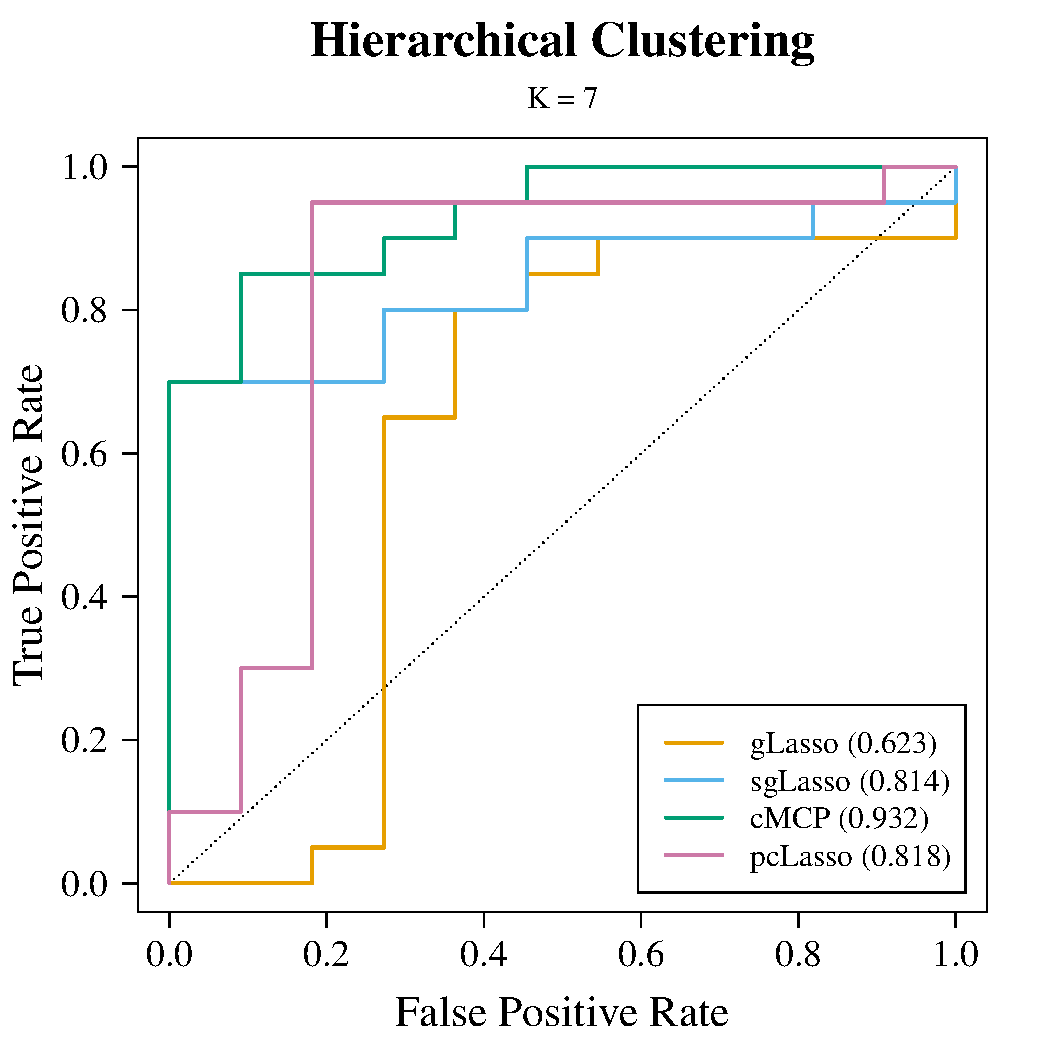
\includegraphics[width = 0.475\textwidth]{colon_ROC_h_n.pdf}
    %\caption{The ROC curves for the colon data set.}
    \label{colon_ROC}
\end{figure}

\end{landscape}
}

%%%%%%%%%%%%% LEUK

\afterpage{
\begin{landscape}
\begin{table}[p]
    \footnotesize
    \centering
    \def\arraystretch{1.5}

    \begin{tabularx}{0.977\linewidth}{lccccccccccc} \toprule
         & \multicolumn{3}{c}{No Clustering} & \multicolumn{4}{c}{$K$-means Clustering} & \multicolumn{4}{c}{Hierarchical Clustering} \\ 
         & \multicolumn{3}{c}{--} & \multicolumn{4}{c}{$K=19$} & \multicolumn{4}{c}{$K=5$} \\   
         \cmidrule(r){2-4} \cmidrule(lr){5-8} \cmidrule(l){9-12}
         % this is what has to be replaced with xtable
         & Lasso & Elastic Net & pcLasso & gLasso & sgLasso & cMCP & pcLasso & gLasso & sgLasso & cMCP & pcLasso \\ \midrule
        \multirow{2}{*}{Parameters} & $\lambda = 0.00407$ & $\lambda = 0.00509$ & $\lambda = 0.00548$ & $\lambda = 0.0779$ & $\lambda = 0.0457$ & $\lambda = 0.111$ & $\lambda = 0.00548$ & $\lambda = 0.0779$ & $\lambda = 0.0236$ & $\lambda = 0.111$ & $\lambda = 0.00548$ \\ 
        & -- &  $\alpha = 0.8$ & $\texttt{rat} = 0.95$ & -- & $\alpha = 0.95$ & $\gamma = 30$ & $\texttt{rat} = 0.9$ & -- & $\alpha = 0.4$ & $\gamma = 30$ & $\texttt{rat} = 0.95$ \\ 
        Deviance & 0.241 & 0.0834 & 0.465 & 1.240 & 0.730 & 0.671 & 0.442 & 1.240 & 0.731 & 0.671 & 0.439 \\ 
        Misclass. & 5/36 & 3/36 & 3/36 & 14/36 & 13/36 & 6/36 & 2/36 & 14/36 & 14/36 & 6/36 & 2/36 \\ 
        Sig. Coef. &  14 &  28 &  41 &   1 &   6 &   6 &  76 &   1 & 772 &   7 &  46 \\ 
        Sig. Groups & -- & -- & -- &  0 &  1 &  2 & 19 &  0 &  1 &  2 &  5 \\ 
        %FPR & 5/14 & 3/14 & 3/14 & 14/14 & 13/14 & 6/14 & 2/14 & 14/14 & 14/14 & 6/14 & 2/14 \\ 
        %TPR & 22/22 & 22/22 & 22/22 & 22/22 & 22/22 & 22/22 & 22/22 & 22/22 & 22/22 & 22/22 & 22/22 \\ 
        AUC & 0.987 & 1.000 & 0.977 & 0.500 & 0.994 & 0.964 & 0.994 & 0.500 & 0.990 & 0.968 & 1.000 \\ 
        %
        \bottomrule
    \end{tabularx}
    \caption{The performance of various models on the leukemia data set.}
    \label{leuk_tab}

\end{table}

\vspace{0.5cm}

\begin{figure}[p]
    \centering
    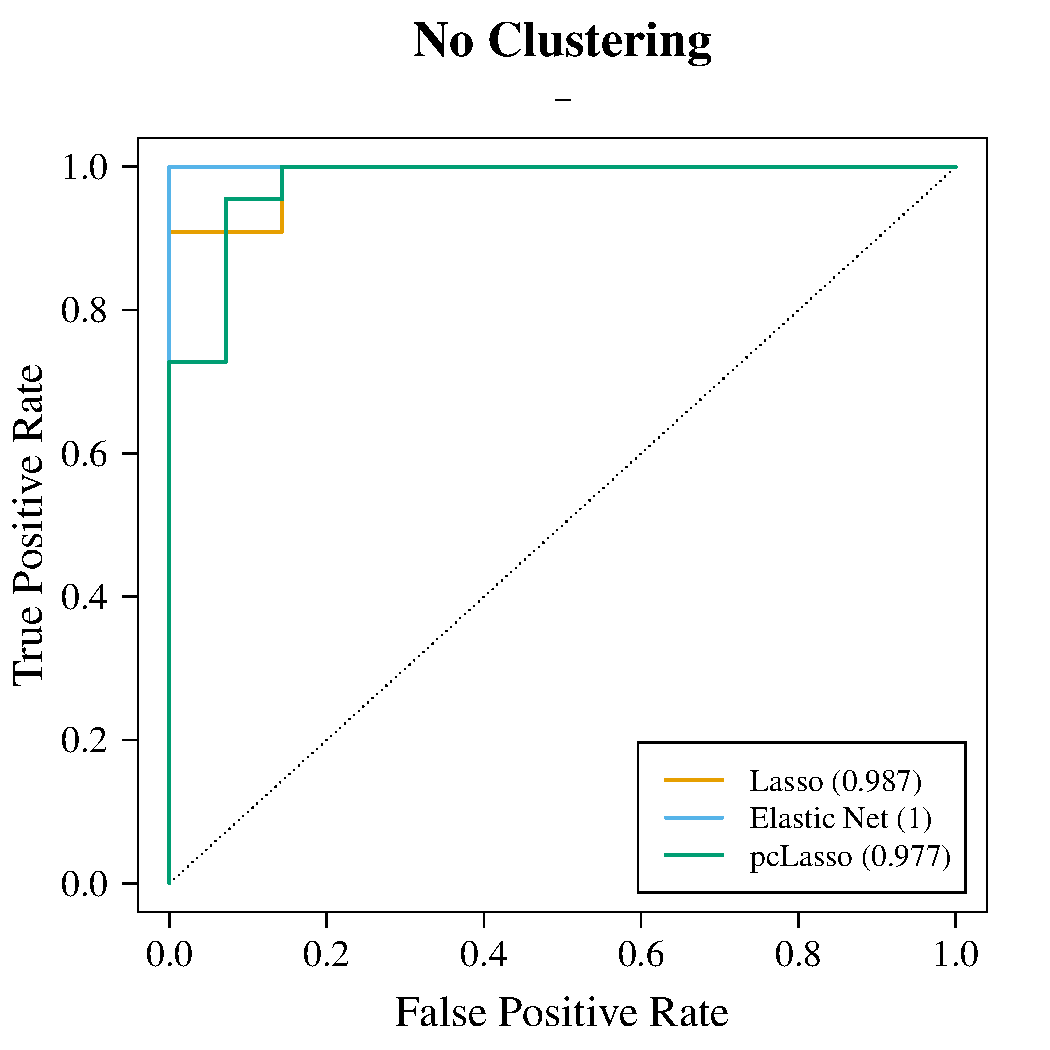
\includegraphics[width = 0.475\textwidth]{leuk_ROC_no_n.pdf}
    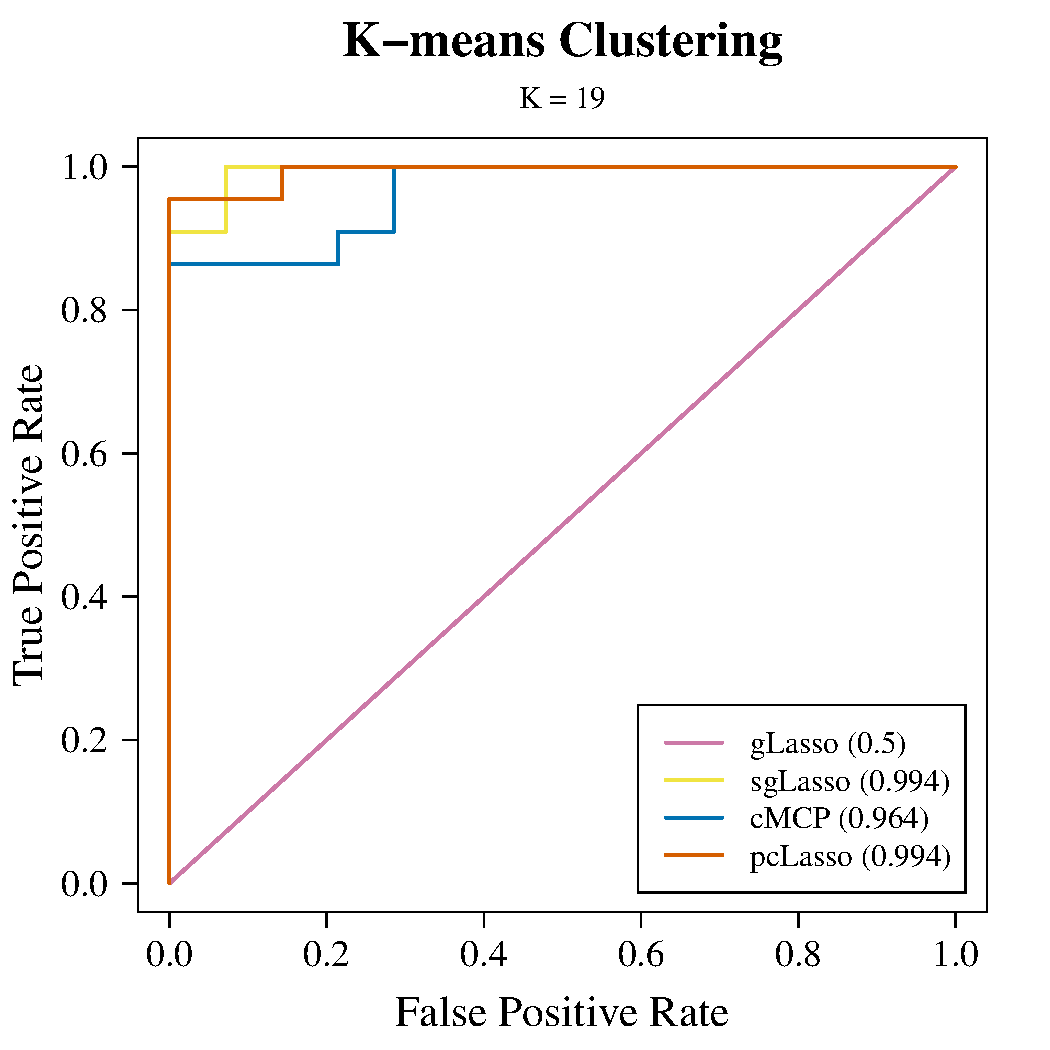
\includegraphics[width = 0.475\textwidth]{leuk_ROC_k_n.pdf}
    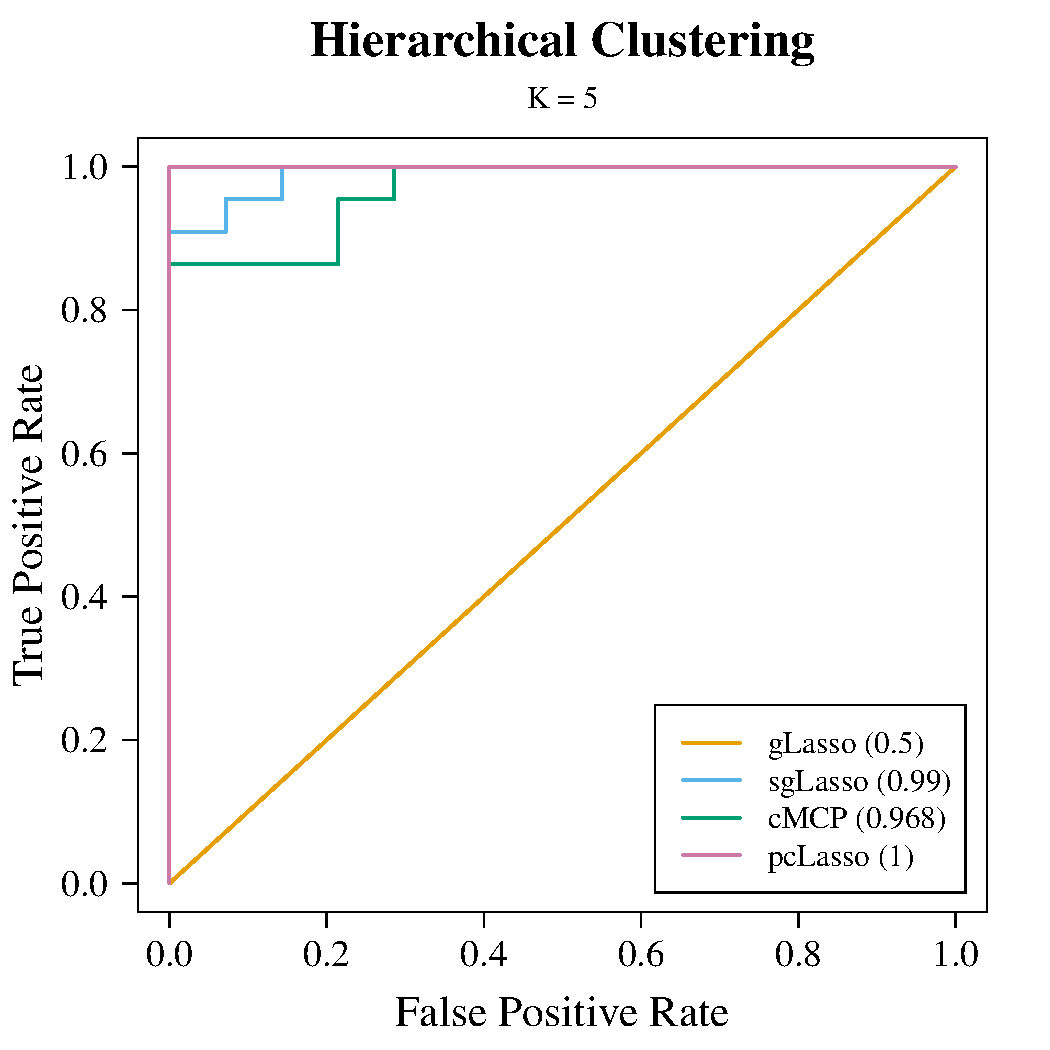
\includegraphics[width = 0.475\textwidth]{leuk_ROC_h_n.pdf}
    \caption{The ROC curves for the leukemia data set.}
    \label{leuk_ROC}
\end{figure}

\end{landscape}
}

\lipsum[3-7]

\end{document}